 \chapter{METHODOLOGY}

        \section{SYSTEM BLOCK DIAGRAM}
            In layman's terms, the home automation project with speech recognition is: you speak into a machine, and it takes that command to control whether household appliances turn on or off as shown in \ref{fig:system1}. 

        \begin{figure}[h]
            \centering
            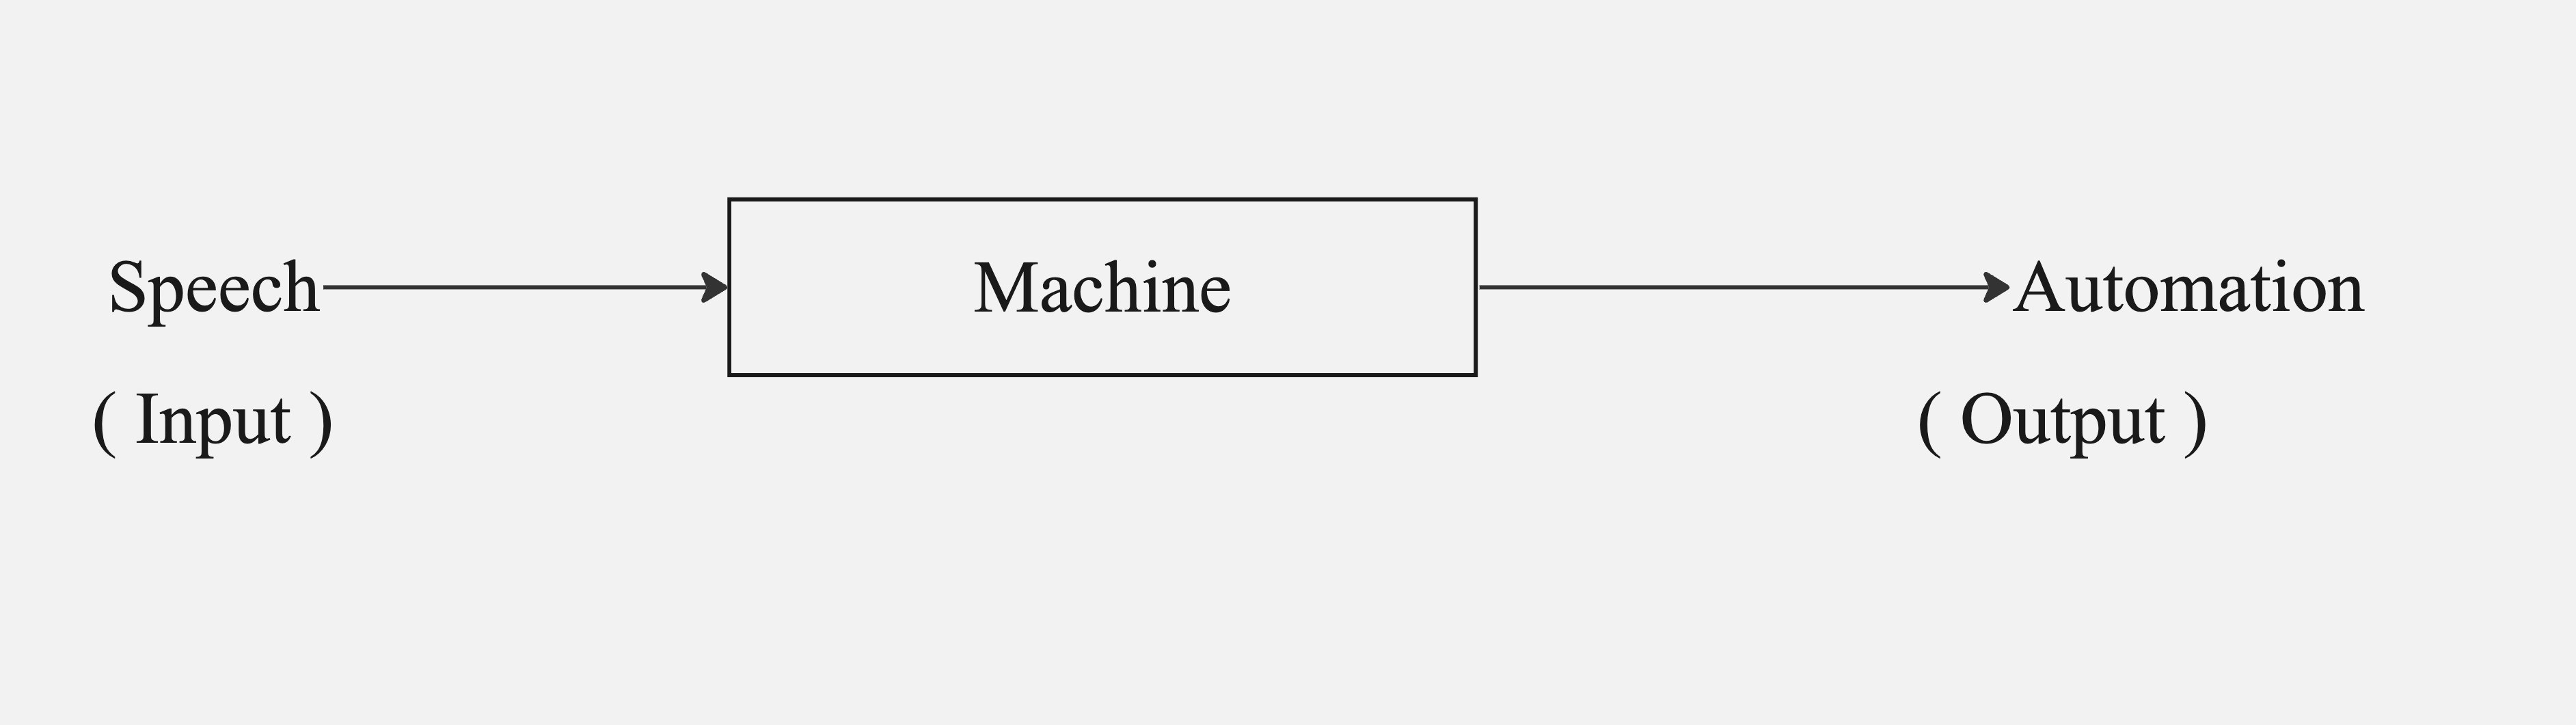
\includegraphics[width=0.9\textwidth]{system1}
            \caption{Block Diagram of Home Automation}
            \label{fig:system1}
        \end{figure}

            Delving deeper into the workings of the system, the process begins with the user providing speech as input through a portable microphone. This input is then transmitted to a Raspberry Pi. Within the Raspberry Pi, a speech-to-text model interprets the spoken words. Upon successful interpretation, the Raspberry Pi generates a signal that commands the control of the appliance(s). This comprehensive system involves multiple components working in tandem to seamlessly translate spoken commands into tangible actions for home automation. The block diagram of the system hardware is shown in \ref{fig:system hardware}.

        \begin{figure}[h]
            \centering
            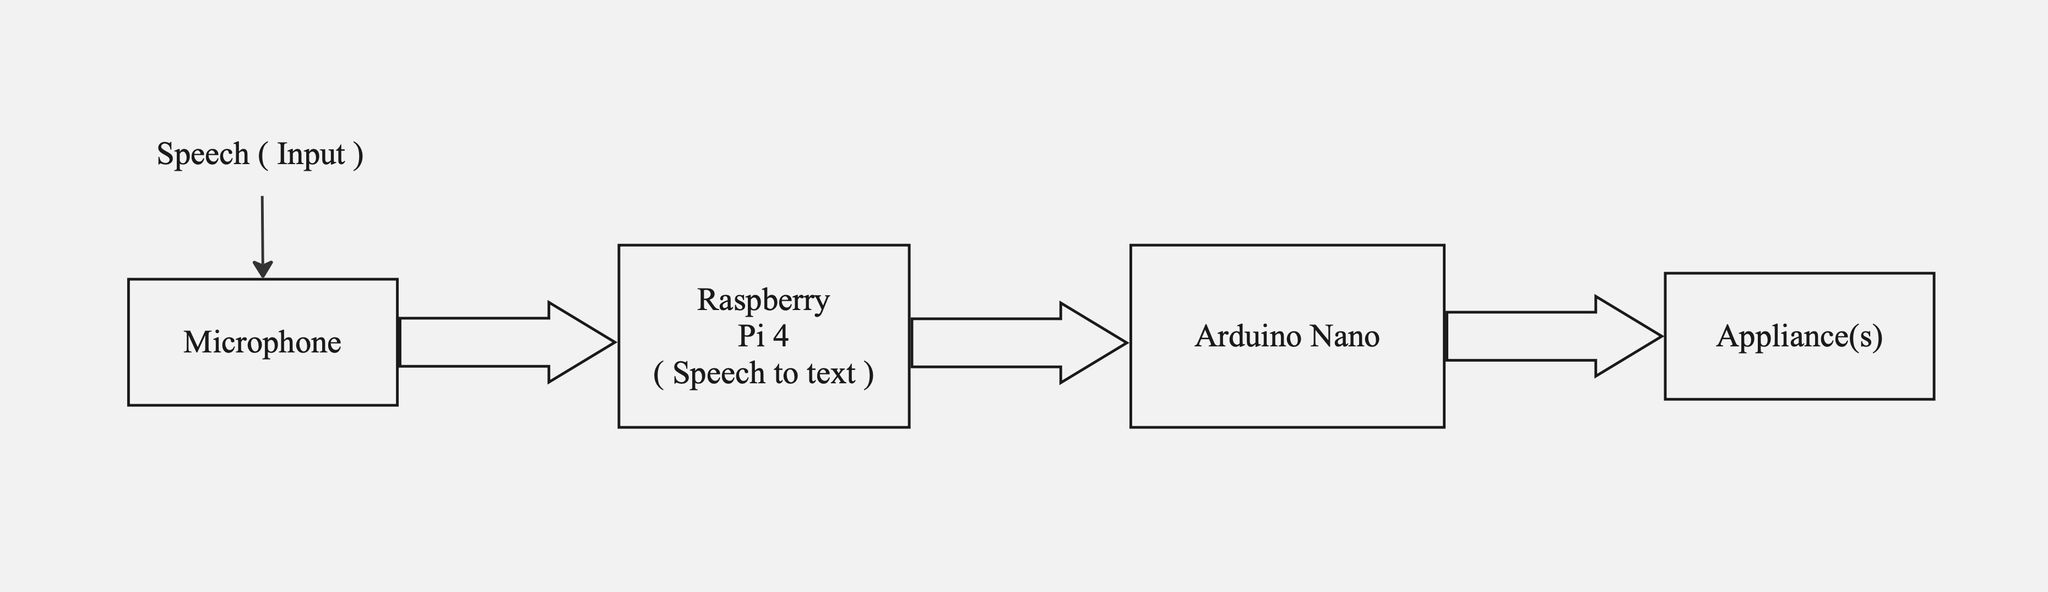
\includegraphics[width=1\textwidth]{system hardware}
            \caption{Block Diagram of System Hardware}
            \label{fig:system hardware}
        \end{figure}

            The process unfolds with the speech serving as input for the speech-to-text model. The converted text undergoes comparison with a wake word in the wake word detector model. If the text does not match a wake word, the system remains inactive until a wake word is detected, prompting the process to restart. Upon recognizing the wake word, the converted text that follows is subjected to a set of conditions, and signals are then dispatched to control the appliances. This iterative sequence ensures that appliance control is contingent on the recognition of a specific wake word, enhancing the system's precision and responsiveness. The flowchart is shown in \ref{fig:system2}.

        \begin{figure}[h]
            \centering
            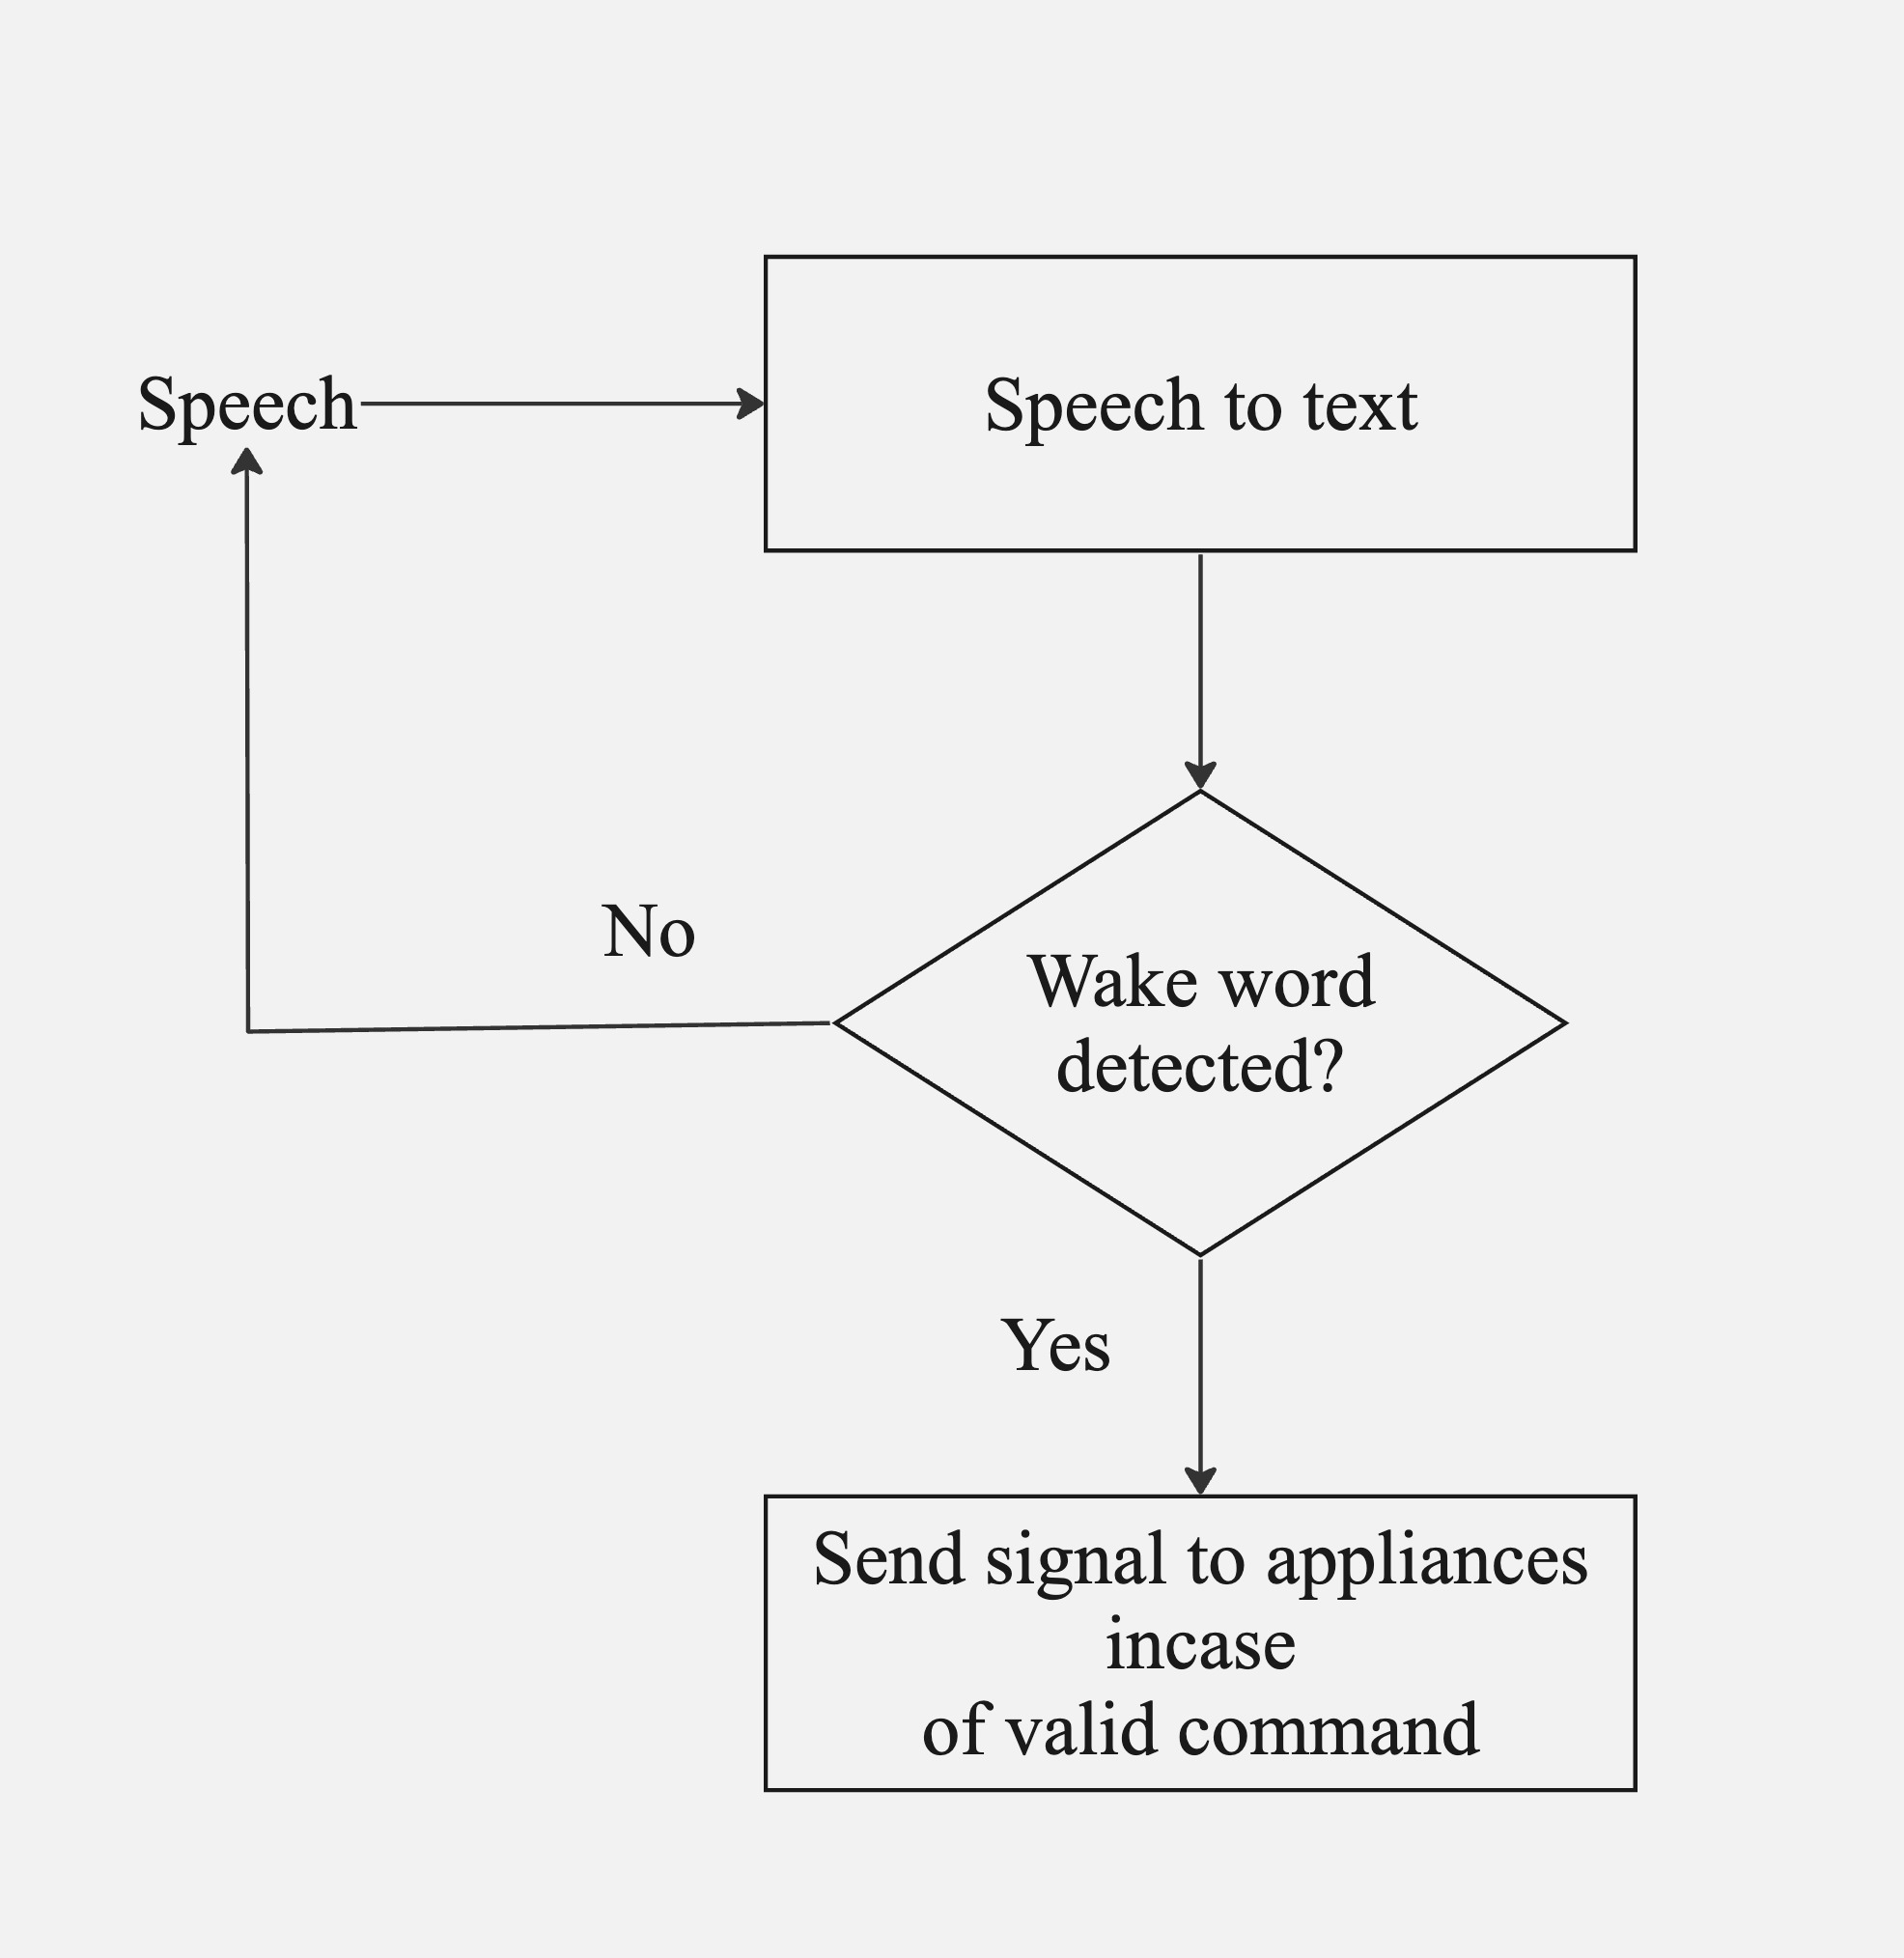
\includegraphics[width=1\textwidth]{system2}
            \caption{Flowchart of Speech Recognition}
            \label{fig:system2}
        \end{figure}
            
       \section{Selection of Raspberry Pi 4 Model B}
       The Raspberry Pi 4 Model B was chosen for our home automation project due to its robust performance, and versatile connectivity. With its quad-core ARM Cortex-A72 processor and adequate memory options, it efficiently executes complex algorithms such as speech recognition. Its built-in Wi-Fi, Bluetooth, USB ports, and GPIO pins facilitate integration with peripheral devices like the Arduino Nano, enabling straightforward hardware control. Overall, the Raspberry Pi 4 Model B serves as the fundamental of our project, offering powerful performance, and reliability to meet the demands of our home automation system.
\newpage
        \section{Activity diagram}
        \begin{figure}[htbp] 
            \centering
            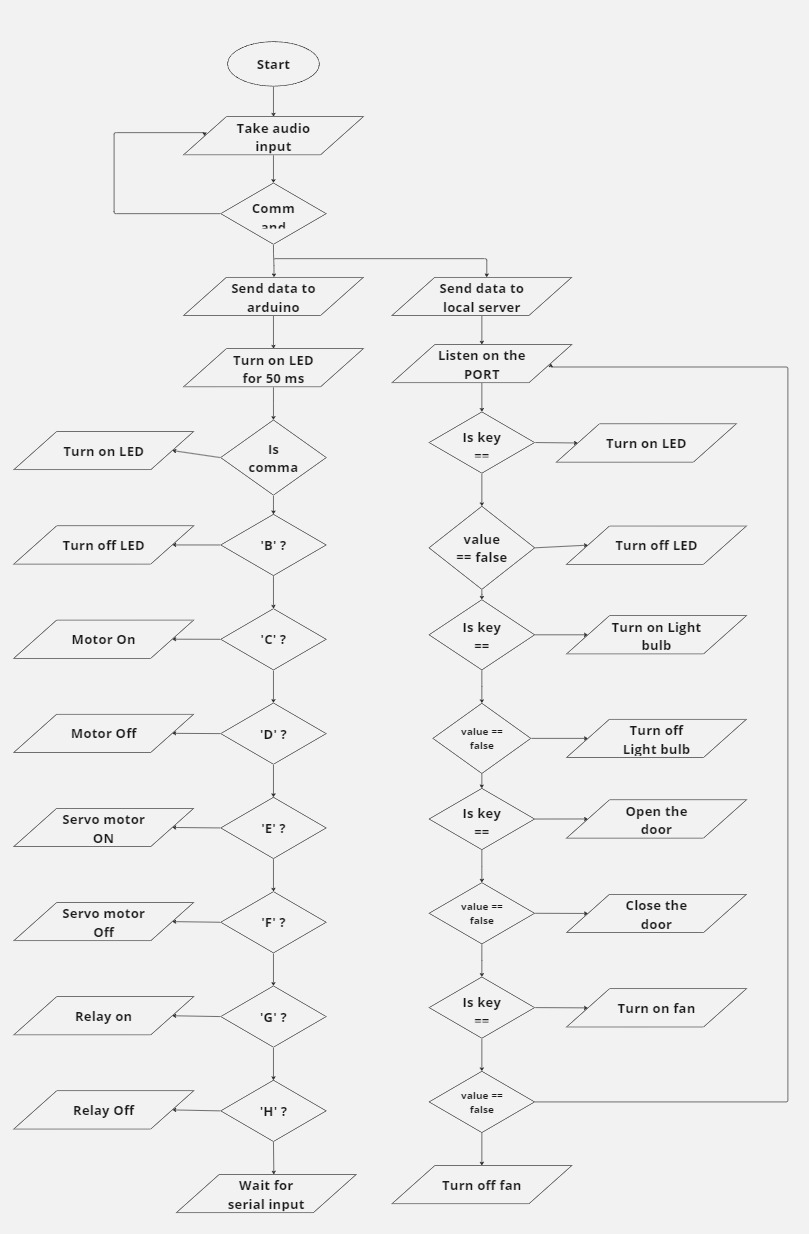
\includegraphics[height=0.7\textheight]{finalact}
            \caption{Activity Diagram}
            \label{fig:Activity}
        \end{figure}
\newpage

        \section{Interfacing between Raspberry Pi 4 Model B and components}
        \begin{figure}[h]
            \centering
            \includegraphics[width=1\textwidth]{interfacing}
            \caption{Interfacing}
            \label{fig:interface}
        \end{figure}
        The Raspberry Pi 4 Model B serves as our development board, which oversees the functions of different hardware elements that, in turn, regulates  the operations of household fixtures. The figure below shows all the interfacing of the home automation system.

        
        From the above diagram, we are illustrating the interfacing between different components present in our system. We are using Raspberry Pi 4 Model B as our development board which uses ARM Cortex-A72 CPU. Control Signal is transmitted from the USB port of the Raspberry Pi to Arduino Nano.The Arduino Nano controls the actions of fixtures. The fixtures are controlled by the signal received from Arduino Nano. External power is provided to the hardware components if needed.\\
        Hence, this is the interfacing between all our components of hardware, i.e Raspberry Pi, Arduino Nano, Relay module, LED, Servo motor, Motor driver and DC motor.

        \section{Interfacing between Hardware and Application}
        The Raspberry pie contains the inbuilt Wi-Fi module which enables the system to come online so a local server is set up. The local server acts as a bridge between the web application and the Raspberry pie. When a command is given to the system then it sends the string to the Arduino Nano via serial communication along with a ‘/post’ request to send the json data for the change in status of the device. Similarly at the website there is a continuous ‘http.get()’ request to fetch the status in realtime, which is then used to change the status of devices in the webpage. Users can see the changes in real time via dashboard.

        \begin{figure}[h]
            \centering
            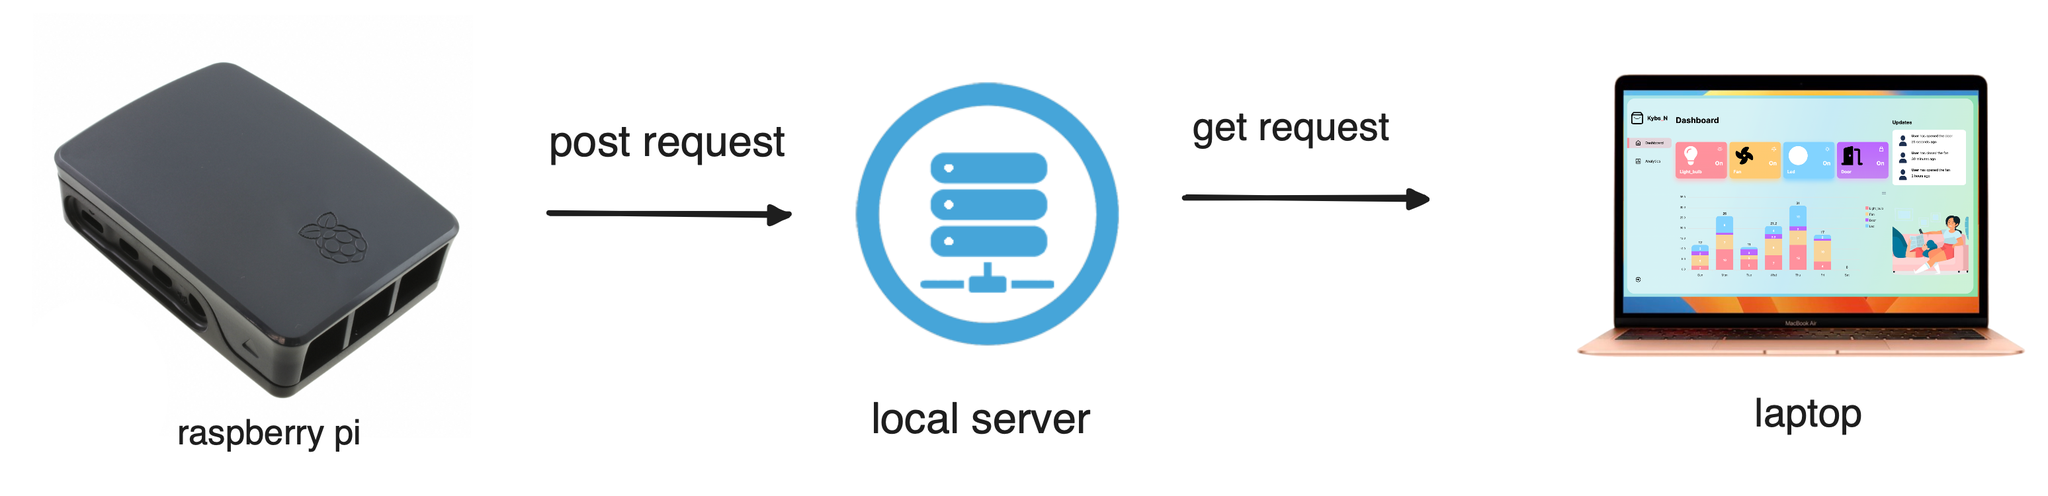
\includegraphics[width=1\textwidth]{hardware_interface}
            \caption{Interfacing between Hardware and Application}
            \label{fig:hardware_interface}
        \end{figure}

        